\glsresetall

\chapter{Introduction}
\label{cha:intro}


Over the last three decades, technological advances have changed the way people use public transport. Before \gls{rti}, travellers would time their arrival at bus stops based exclusively on the bus's scheduled arrival time. There was no way of knowing if the bus was on-time, running late, or indeed if it was on its way at all until it bus finally appeared around the corner. These days, however, travellers can check the location of a bus from their phone before even leaving home. Despite the accessibility of such \gls{rti}, unforeseeable traffic situations and various bus behaviours make
estimating arrival times from vehicle locations a difficult task.


Around the world, public transport providers have invested in systems to provide \gls{rti} to travellers. Research has found that the experienced wait time of travellers is shorter (versus their actual wait time) when an arrival time countdown is displayed at the stop \citep{TCRP_2003}. Further, \citet{Cats_2015} and \citet{Lu_2017} each reported that passengers who use \gls{rti} actually have shorter wait times, on average, than those who do not. Of course, if \glspl{eta} are unreliable, passengers instead get frustrated. Improving the \emph{reliability} of \gls{rti} is therefore crucial for improving \emph{ridership} (the number of passengers using public transport).


One limitation of \gls{rti} is the infrastructure required to keep track of vehicles and relay information to commuters \cite{TCRP_2003b}. As fleet sizes increase (over 1000 in Auckland), so do the demands of the \gls{atis}, which has led some providers, notably Auckland Transport, to use the simplest of arrival time prediction frameworks. This simplification consequently results in less reliable systems, as I will discuss in \cref{sec:auckland_etas}.


The history of \gls{rti} for public transport spans several decades, which we will now examine, focussing on the key concepts essential for reliable \glspl{eta}. Afterwards, the current state of arrival time prediction in Auckland, New Zealand is examined to establish why---despite decades of research---there is room for significant improvement. Finally, I present the aims of this research and summarize the process of estimating the arrival time of buses.



\section{A brief history of real-time information}
\label{sec:literature}

For a long time, public transport services such as buses and trains had only static timetables that passengers would use to plan their journey. There was no way for passengers to know if their bus was on-time, late, or early, nor could operators track how their services were running. In the 1960s, the first vehicle tracking systems were trialled in Germany and the United States of America \citep{TCRP_1997}. These early systems used \emph{beacons} (on signposts) placed along the route that the bus detects, allowing the bus to provide its location to the service provider in real-time. Similar vehicle tracking technologies continued to develop over the subsequent decades, but the focus remained on service monitoring and operational control.


The earliest uses of \gls{avl} technology for passenger information were \glspl{dms} at bus stops displaying a countdown to the next bus's arrival \citep{TCRP_2003}. One early example of this was Transport for London's \emph{Countdown} system \citep{Balogh_1993}, which used the beacon (or signpost) \gls{avl} technology in conjunction with vehicle odometers. The system was able to determine vehicle locations and predict arrival times at stops.


Other vehicle tracking methods have since emerged using a range of technologies, such as odometers, but the most notable is the widely used \gls{gps} \citep{Zhao_1997}. One significant advantage of the \gls{gps} is that it does not need any fixed infrastructure (such as signposts along the route), making it easy for transit providers to add new routes or reroute existing ones without breaking the \gls{avl} system. A disadvantage of the \gls{gps} is that, rather than receiving \emph{route-specific} positions (``Signpost 8'', for example) the observations are \emph{map coordinates} which require an additional step to match them to the route.\footnote{Route matching and the issues associated with it are discussed in depth in later chapters.}


\citet{Cathey_2003} proposed a general prescription for making real-time arrival time estimates from \gls{gps} vehicle location data consisting of three components. First, a \emph{tracker} matches observations to scheduled \emph{trips} (time-specific instances of a route), which involves mapping \gls{gps} observations to the \emph{route path} to calculate the bus's \emph{trip-distance-travelled} (the distance the bus has driven along the route). Second, a \emph{filter} estimates the underlying vehicle state (including speed) which is updated, in real-time, as new observations are received. \Citeauthor{Cathey_2003} used a Kalman filter for this step due to its superior real-time performance and previous use for modelling transit vehicle state \citep{Wall_1999,Dailey_2001}. In the final \emph{prediction} component of their prescription, \citeauthor{Cathey_2003} used the estimated vehicle state in conjunction with travel time forecasts (estimated from historical data) to predict \emph{time until arrival}.


Other \gls{avl} systems report the vehicle's arrival and departure times from \emph{time points} (which are usually a subset of specific stops), providing observations of travel time between them. This type of reporting led to a range of new methods of arrival time prediction. For example, \gls{ann} and \gls{svm} models were implemented to predict travel time \citep{Jeong_2005,Shalaby_2004,Yu_2011,Cats_2015,Cats_2016,Yin_2017}. Many of these were in-depth research projects with access to high-quality data, such as high-frequency polling (10~seconds of less) or video footage to calculate, for example, precise arrival and departure times. Despite their differences, all of their methods specify the importance of two components to arrival time prediction: \emph{travel time} between stops (or time points), and \emph{dwell time} (time spent servicing a stop).


The concept of travel time between time points forms the foundation of arrival time estimation, so the estimation or even forecasting of travel times has been the focus of much research. Returning to Transport for London's \emph{Countdown} system, \citet{Reinhoudt_1997} stored real-time travel time between time points and stored them in a database. They then used a \kf{} to update link travel times, improving the accuracy of arrival time prediction. Others, such as \citet{Wall_1999}, \citet{Dailey_2001}, and \citet{Cathey_2003}, used historical data to estimate \emph{time until arrival} given a vehicle's trip-distance-travelled and speed. Further improvements to prediction accuracy were obtained when real-time travel time along links were updated using a \kf{}, which was capable of reacting to changes in traffic \citep{Shalaby_2004}.


Other models used for arrival time prediction include \gls{ann} and \gls{svm}. \Citet{Yu_2006} demonstrated the feasibility and applicability of using an \gls{svm} to predict travel time based on the current segment travel time and the travel time of the most recent bus servicing the same route along the next segment. The limitation was, of course, that the model was trained for only one single route and only provided an arrival time for the next time point. Later, \citet{Yu_2010} proposed an improved hybrid model using an \gls{svm} to model baseline travel time and a \kf{} to incorporate real-time data. Their method was again limited to a single route and single-interval, but demonstrated the importance of using real-time information for arrival time prediction. The next significant result was from \citet{Yu_2011} when they demonstrated the use of data from multiple routes to predict arrival time. In their study, \citeauthor{Yu_2011} used the travel time of recent buses between an automatic toll reader and a specific bus stop. While not generalised, they demonstrated the advantage of combining data across routes.


\Citet{Yin_2017} presented a model to predict travel times between stops using travel times of previous buses from multiple routes, in which they chose two overlapping routes and manually identified common stops. They were able to predict travel time reasonably well, though both their \gls{svm} and \gls{ann} models failed to capture the peak period congestion. An alternative to machine learning models was proposed by \citet{Chen_2014}, who used a \emph{particle filter}\footnote{Their particle filter is unrelated to ours, but the general methodology is the same and described in \cref{sec:recursive-bayes}} to predict car travel time along roads from a database of historical data. Another unique approach by \citet{Julio_2016} used the concept of \emph{traffic shock waves} to predict travel times of buses along links based on the travel time along adjacent links. They used \gls{gps} observations to calculate vehicle trajectories over time, and developed an \gls{ann} to learn patterns: as congestion builds along a segment, so too does congestion along the segment before it, for example.


Most of the methods described above only provide predictions for travel time along the next link, so arrival times are not available for stops further down the route. \Citet{Chang_2010} developed a \gls{knn} algorithm trained on historical vehicle trajectories. They predicted travel time along multiple upcoming links along a single route both accurately and efficiently (their method could make 4000~predictions per minute).


Since travel time of previous buses had been shown to improve arrival time predictions, other sources of information were explored to further improve prediction accuracy. This could be important along roads with low-frequency trips or subject to fast-changing traffic conditions. \Citet{Xinghao_2013} and \citet{Ma_2019} incorporated real-time taxi data to model traffic state. While this showed improvements, it is clearly limited to locations with open access to taxi data.


Another source of uncertainty in arrival time comes from \emph{dwell time} at stops. That is the time spent by the bus at stops while passengers board and disembark. \Citet{Shalaby_2004} showed that dwell times can have a massive influence on arrival times. Along with a \kf{} for link travel times (each link consisted of 2--8~stops), \citeauthor{Shalaby_2004} also implemented a \kf{} on stop dwell times, allowing them to respond to real-time demand fluctuations which they measured using \glspl{apc}. Other work has also demonstrated the necessity of incorporating dwell times into arrival time predictions \citep{Jeong_2005,Cats_2015,Cats_2016}.


When it comes to modelling transit vehicles and predicting arrival times, there is a lot of uncertainty in vehicle trajectories, particularly when observations are sparse, and much of this uncertainty is non-Gaussian (particularly multi-modal). \Citet{Hans_2015} presented a particle filter for modelling transit vehicles. Their model incorporated bus stop dwell times and traffic lights, and their data came from \gls{gps} and \glspl{apc}. The primary advantage of the particle filter over other methods (such as the \kf{}) is that it is capable of sampling a wide range of plausible trajectories. This is particularly important when forecasting multiple stops ahead, when the level of uncertainty increases significantly.


Since uncertainty is an unavoidable component of arrival time prediction, some attempts at conveying this to travellers has been explored. \Citet{Mazloumi_2011} assessed the use of \emph{prediction intervals} obtained from an \gls{ann} model, focussing on the accuracy (coverage) of these intervals. A more unique approach was demonstrated by \citet{Fernandes_2018} that involved displaying \emph{uncertainty graphs}---including quantile dot plots---and found that their test subjects made better decisions when they had uncertainty information, as opposed to singular point estimates.


The final component of \gls{rti} that we are interested in is \emph{journey planning}, which involves the selection of an optimal route to get to a destination, often under one or more constraints. \Citet{Horn_2004} developed a real-time routing method that could incorporate \emph{walking} and \emph{waiting costs} (each of these should be minimised where possible), with a focus on \emph{demand-responsive} services. More recently, \citet{Hame_2013a,Hame_2013b} proposed a \emph{Markov decision process} which could maximise the probability of arriving to the destination on-time, accounting for walking legs and distributions for the arrival time of buses at stops. Travel time uncertainty was incorporated into the method used by \citet{Zheng_2016}, who also demonstrated the complexity of the problem, which could take $10^3$~seconds to find an optimal route; their solution was to store paths, which reduced the computation to less than a second. As an alternative to incorporating travel time uncertainty, \citet{Berczi_2017} propose a dynamic routing strategy that uses any probabilistic model of arrival and departure times, and improved the probability of arriving at the destination on time.



\section{The state of Auckland's \gls{rti}}
\label{sec:auckland_etas}

Our principal case study is the public transport system in Auckland, New Zealand, operated by Auckland Transport. In the following pages, I describe some scenarios that occur within Auckland\footnote{Some of which I have personally witnessed.} although they likely occur in other cities that use the same infrastructure (described in detail in \cref{sec:gtfs}). Additionally, Auckland has a lot of locations without transit infrastructure, such as bus priority lanes, which can lead to long delays during heavy congestion.


Other issues relate to driver behaviour and \emph{schedule adherence}. There is also no incentive for drivers to actively adhere to the schedule, as ``Punctuality is measured by the percentage of total scheduled services leaving their origin stop no more than one minute early or five minutes late'' \citep[13]{AT_report_2019}. As demonstrated in \cref{fig:schedule_adhere}, buses tend to run early, particularly towards the end of the route, which I would argue is more frustrating than running late for anyone wanting to catch it. At other times, travellers may need to catch multiple buses to get somewhere, in which case a \emph{transfer} between services is necessary. However, if the first bus runs late, the connecting bus will usually depart on time (before the first bus gets there) leaving the passenger stranded until the next trip. In some cases, this may be 30~minutes or more, which inevitably leads to frustrated passengers.\footnote{I have been most unfortunate to watch a bus depart without me just as the one I'm on pulls into the station on more than one occasion.}


\begin{knitrout}\small
\definecolor{shadecolor}{rgb}{0.969, 0.969, 0.969}\color{fgcolor}\begin{figure}
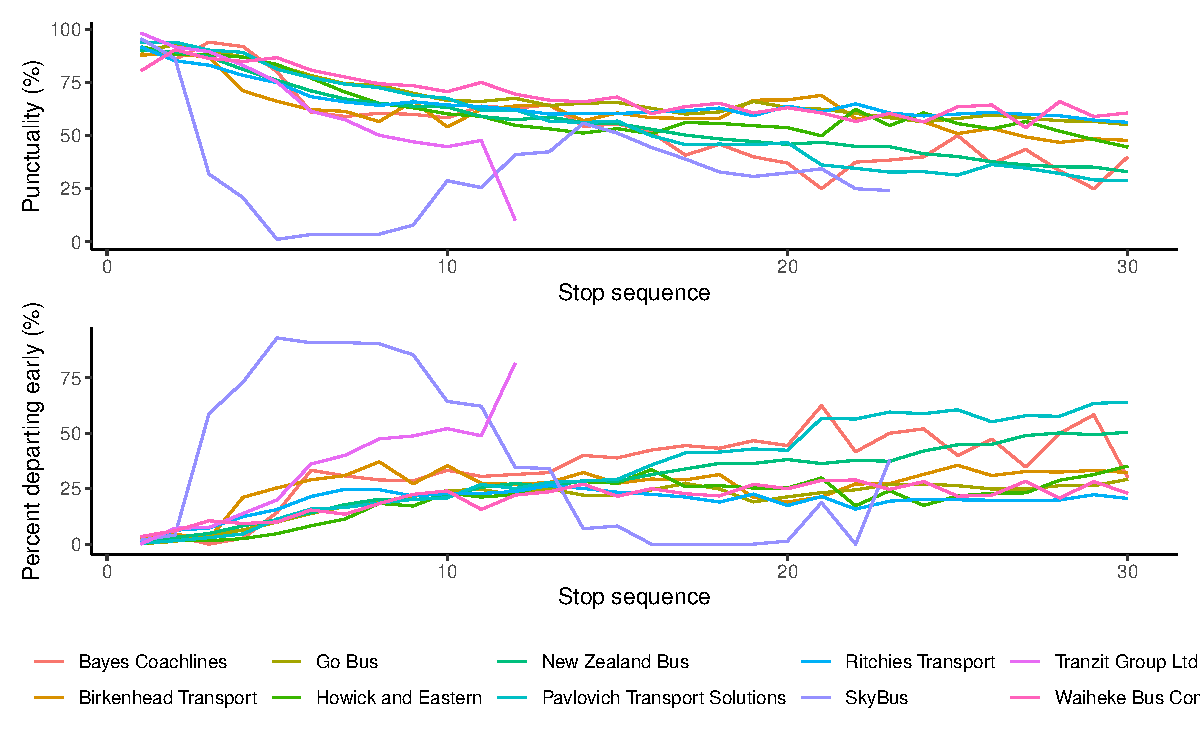
\includegraphics[width=\linewidth]{figure/schedule_adhere-1} \caption[Punctuality of various providers in Auckland (departing between 1 minute early and 5 minutes late), and also the percent departing early]{Punctuality of various providers in Auckland (departing between 1 minute early and 5 minutes late), and also the percent departing early.}\label{fig:schedule_adhere}
\end{figure}


\end{knitrout}



Given that many of the issues with Auckland's transport system relate to infrastructure, the easiest solution is improved, reliable \gls{rti}. Auckland Transport uses \gls{gtfs}, a specification for how transit data should be organised \citep{GoogleDevelopers_2006}. Part of \gls{gtfs} provides a simple method for predicting arrival times, which is what Auckland Transport and other agencies use. In this method, \emph{trip updates} are reported when a bus arrives or departs from a stop, and includes the vehicle's \emph{delay} (the difference between scheduled and actual arrival). Arrival time at upcoming stops is then estimated by adding this delay to the scheduled arrival time. While this is simple, it quickly runs into problems, particularly if the scheduled travel times are not accurate and drivers do not actively adhere to them.


Besides being inaccurate and unreliable, arrival times based on schedule and current delay are prone to sudden changes in the vehicle's delay. For example, if the bus encounters heavy traffic between stops, it will get a lot later, but this is not reported to passengers until the bus finally arrives at the next stop, in which case passengers waiting at stops further along see the \gls{eta} suddenly increase. Another common occurrence is when the bus is delayed on a previous trip: the default arrival time estimate is the scheduled arrival time, so until the bus starts the trip, the \gls{eta} is as scheduled. When the bus is delayed, it may start the route 10~minutes late. When it does, all the \glspl{eta} at stops will suddenly increase by 10~minutes; however, if the \gls{eta} reaches zero before the bus commences the trip, the bus disappears from the \gls{dms} completely. These scenarios all contribute to traveller frustration and lack of trust in the system.


Conversely, \gls{gtfs} provides an opportunity for a standard, globally available framework: ``The standardised format means that innovative tools and products that utilize GTFS can easily be applied across transit agencies.'' \citep[26]{TCRP_2020}. It is therefore desirable to have a framework based around \gls{gtfs} that is capable of using the available data (both static and real-time) to model transit vehicles, estimate traffic conditions throughout the network, and estimate arrival times. Location-specific features, such as taxis or intersection locations, could be added as necessary provided the framework is structured to allow it.


The core components described in the literature as essential to arrival time prediction are travel time and dwell time. To the best of our knowledge, no system exists that bases itself purely on \gls{gtfs} data while providing a means of combining data across routes to estimate traffic conditions which can be used to improve arrival time prediction.



\section{Research proposal}
\label{sec:proposal}

Public transport is essential wherever people need to get to and from work, school, or other activities dependably. However, in this age of cellphones and \gls{rti}, travellers have come to expect, at the very least, the countdown on the \gls{dms} at their stop to be reliable---in Auckland, this is not the case. This unreliability makes \gls{eta} unusable for real-time journey planning, making it difficult for commuters to rely on public transport and opt instead for alternative, often private, transport options.


The central focus of this thesis is the development of an arrival time prediction application that includes real-time traffic information obtained from both static and real-time data using \gls{gtfs}. This means that the application can be applied to any city using \gls{gtfs}, and not solely Auckland, as many of the problems discussed earlier will be present elsewhere. This involves exploring how traffic state can be estimated independently of routes so that travel time or speed information can be shared across routes that use the same roads. Our goal is to make arrival time predictions which, by accounting for real-time traffic conditions, are more reliable that the current method used in Auckland. However, it is clear from both the literature and personal experience that large levels of uncertainty are inescapable in transit prediction. For this reason we focus on capturing the uncertainty in the model and estimating the \emph{arrival time distribution}, which we can then summarize with, for example, prediction intervals.


We also consider journey planning, notably the use of arrival time distributions to make decisions, since Auckland (and other) transit providers offer no such service: all the ``journey planning'' is based solely on the scheduled timetables. \Citet{Berczi_2017} demonstrated the use of probabilistic arrival time distributions in a real-time dynamic routing problem. It is not our intention to solve the routing problem (that is, selecting candidate routes from origin to destination), but instead to demonstrate the reliability (or usefulness) of our own arrival time distribution in selecting between alternative routes. This could then be incorporated into a dynamic routing framework that uses the probabilities of events to make decisions.


Before approaching this problem, I first provide an overview of the relevant background information in \cref{cha:data}. This includes an overview of \gls{gtfs}, and discuss the characteristics of real-time transit data. We will also examine how a \emph{network} can be constructed from \gls{gtfs} data to allow data to be shared across independent routes. Lastly, I give a brief introduction to \emph{recursive Bayesian filtering}, an approach to modelling data in real-time that is used extensively throughout this thesis.


Having placed some foundations, we begin the process of real-time prediction by first modelling the state of a transit vehicle, which will be updated whenever new data is received. One important aspect of this chapter involves removing all unnecessary uncertainty. \Citet{Cathey_2003} (and others) used \emph{map-matching} to calculate the vehicle's trip-distance-travelled from the reported \gls{gps} coordinates. In \cref{cha:vehicle_model}, as part of the vehicle model, I propose a method of removing this step and incorporating \gls{gps} observations directly into the likelihood function in an effort to overcome several of the issues identified in \cref{cha:data}. The main goal of \cref{cha:vehicle_model} is to use real-time transit vehicle observations to estimate vehicle speed along road. This is similar to the work of \citet{Celan_2017,Celan_2018} who used historical data to estimate average vehicle speed along roads in a \emph{network}.


Having observed the speeds of vehicles as the travel around Auckland, we can model the real-time \emph{traffic state} of the road network. Similar to the work of \citet{Shalaby_2004} we develop a \kf{} that allows real-time estimation of network state in \cref{cha:network_model}. A large part of this consists of estimating the necessary model parameters from historical data and assessing the real-time accuracy of our model. As many previous researchers have noted, predicting future travel times (which depend on road state) is difficult and requires a more complex model than the \kf{}. At the end of \cref{cha:network_model} I discuss a possible approach to forecasting that could later be incorporated into the arrival time prediction component of our application.


Finally, we arrive at arrival time estimation itself, which combines vehicle and road states to obtain an arrival time distribution. In \cref{cha:prediction}, we see how the distribution itself is computed, and compare our approach to several others, with a focus on the adequacy of the distribution since, as we have already mentioned, uncertainty is inevitable. Later in \cref{cha:etas} I demonstrate how an arrival time \gls{cdf} is obtained, and present several forms of summary statistics that could be displayed to commuters (point and interval estimates), as well as demonstrate the use of the distribution to answer journey planning questions (journey length, probability of on-time arrival, and the likes). The focus of these results is a comparison of the reliability and potential usefulness of our method versus that currently used in Auckland.


Since this is a real-time application, the computational constraints are also assessed throughout. Therefore, at the end of each chapter, I describe the programmatic considerations of the application and discuss the relative components of the R package `transitr` developed as part of this research. The target for real-time predictions---from the time the data is first requested from the server until \glspl{eta} are available for travellers---is 30~seconds.


Finally, in chapter 7, we review our methods and findings and comment on what could be done to improve our application in the future. The role of \gls{rti} in public transport is only going to become more critical as cities---particularly Auckland---grow, and improving the reliability of the information is the first step to increasing ridership.
